\newpage
\section{Vorgehen}
Es wurde beschlossen, nach SODA \cite{Wikipedia-Scrum} vorzugehen.
SODA ist eine einfache und agile Vorgehensweise zur Entwicklung von Projekten. Dieses Vorgehensmodell wurde von der Hochschule Luzern entwickelt, um den Studenten eine iterativ/inkrementelle Vorgehensweise zu bieten, welche trotzdem zeitlich begrenzt ist. Somit ist es eine Mischung aus dem Wasserfallmodell und Scrum. Scrum wird häufig in der Software Entwicklung eingesetzt, wurde aber ursprünglich aus Studien von Manufakturen wie der Autoindustrie entwickelt \cite{Wikipedia-Scrum-History}.

Da es sich in \acrshort{pren1} nicht um ein reines Software-, sondern um
ein Interdisziplinäres Projekt handelt, besteht die Gefahr, dass Aufgaben
mit niedrigerer Priorität nicht umgesetzt werden. Aus diesem Grund ist es
wichtig, bereits im Vorhinein mögliche Risiken zu identifizieren und deren Machbarkeit
abzuklären. Dies wurde mittels \nameref{sec:design-thinking} gemacht.

Um zu vermeiden dass niedriger priorisierte Aufgaben nicht vernachlässigt werden,
ist es wichtig ein gutes Backlogmanagement zu erstellen. Das heisst alle Aufgaben/Stories zu definieren (siehe \ref{tab:anforderungsliste}), zu schätzen und zu priorisieren. Damit kann bereits früh festgestellt werden, welche Aufgaben zeitlich umgesetzt werden können.

Es werden wöchentliche Stand-Ups mit dem Coach und allen Teammitgliedern durchgeführt, hierbei wird besprochen, was in der letzten Woche erreicht wurde, was für Risiken und Hindernisse bestehen (siehe \nameref{sec:risikomanagement}) und was bis zum nächsten Stand-Up erreicht werden soll.

Als Scrum-Board wird Trello\footnote{https://trello.com/} verwendet.

\subsection{Organigram}
SODA gibt die folgenden Rollen vor:

\begin{items}
  \item {\bf \acrfull{po}} \\
    Repräsentiert die Kunden des Produktes gegenüber dem Team 
    und ist verantwortlich um einen Business-Value zu generieren.
  \item {\bf \acrfull{sm}} \\
    Entfernt Hindernisse, die das Team an der Producktentwicklung hindern.
  \item {\bf Entwicklungsteam} \\
    Ist für die Entwicklung des Producktes zuständig
\end{items}

\newpage

Die Rollen wurden gemäss dem Organigramm in Abbildung \ref{fig:organigramm} auf das Team verteilt. Natürlich sind im Rahmen der \acrshort{pren1} Arbeit alle Teammitglieder teil des Entwicklerteams.
Je nach Rolle kann aber mehr oder weniger Arbeit beispielsweise für das Backlogmanagement anfallen.

\begin{figure}[H]
  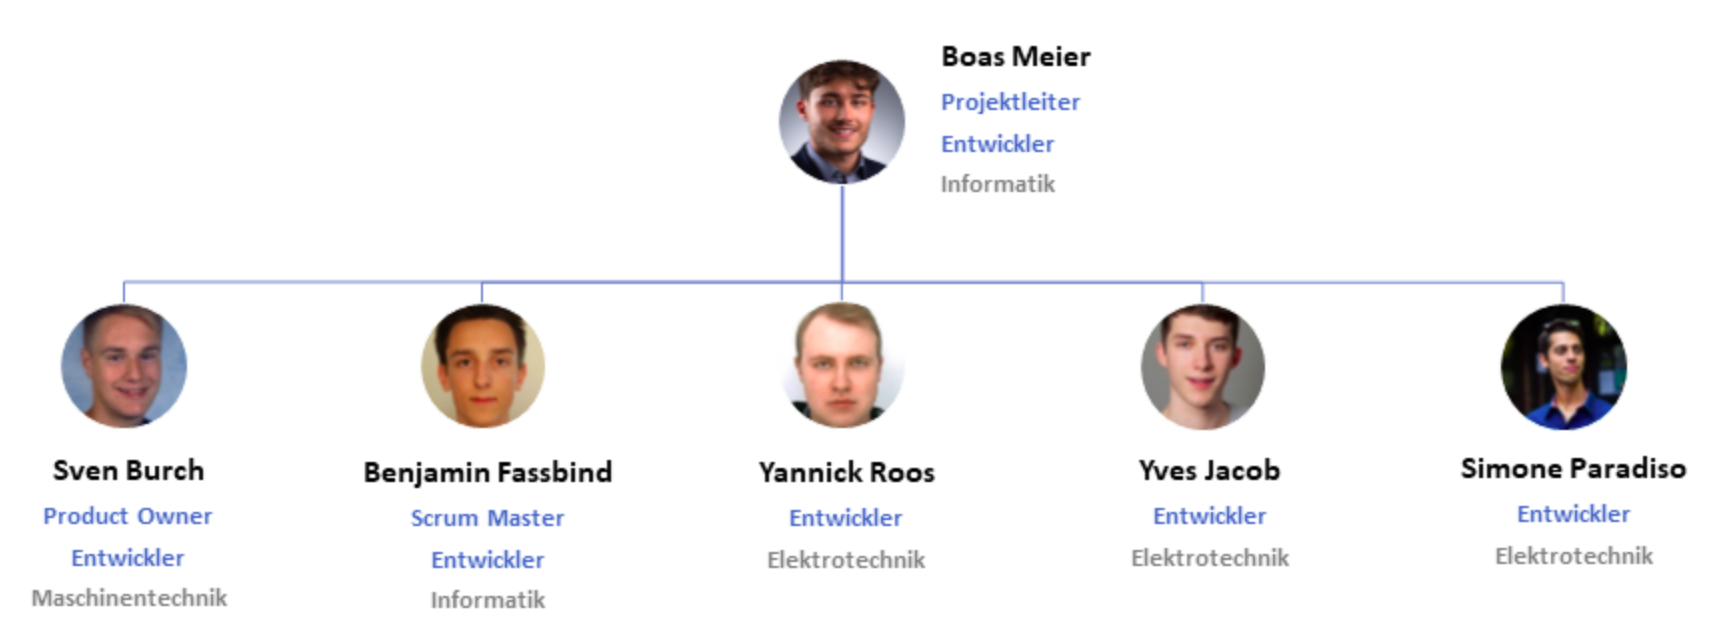
\includegraphics[width=1.0\textwidth]{img/organigram}
  \centering
  \caption{Organigram welches die Projektrollen festlegt}
  \label{fig:organigramm}
\end{figure}

\subsection{Datenaustausch}
Um Daten im Team auszutauschen und gemeinsam Dokumente zu erarbeiten, werden zwei verschiedene Cloud Plattformen verwendet. Jedes Teammitglied hat vollständigen Zugriff auf beide Plattformen.

\textbf{OneDrive}\\
Microsoft OneDrive wird verwendet, um Office 365 Dokumente zu verwalten. Dank OneDrive sind diese Dokumente versionskontrolliert und unter allen Mitgliederen synchronisiert. Dies erlaubt eine simultane Bearbeitung.

\textbf{GitHub}\\
Mit Hilfe von GitHub wird der Quellcode versionskontrolliert verwaltet. Es wurden zwei Repositories angelegt. Die \LaTeX-Dokumentation ist unter dem Repository https://github.com/randombenj/hslu-pren1-doc erreichbar und der Quellcode unter https://github.com/randombenj/hslu-pren1.

\newpage

\subsection{Design Thinking}
\label{sec:design-thinking}


Bei Design Thinking \cite{Wikipedia-Design-Thinking} geht es in erster Linie darum, strukturiert 
Ideen für die Umsetzung eines neuen Produktes zu finden. Auch soll das Design Thinking
dabei helfen, zu sehen, ob eine Idee umsetzbar ist. Dies wird dadurch erreicht,
dass sehr einfache (\acrshort{lofi}) Prototypen, beispielsweise aus Karton, 
gefertigt werden, um zu sehen, ob das gewünschte Konzept überhaupt umsetzbar ist.

Ein Ansatz des Design Thinking ist der Double Diamond Prozess. Auch dabei geht es
darum, dass man mit einem Problem konfrontiert wird, im hier dargelegten Fall durch die 
Aufgabenstellung, und versucht dabei die bestmögliche Lösung zu finden.

Die Idee dabei ist relativ einfach: Man unterteilt die Problemlösung in vier Teile.
Als erstes versucht man, möglichst breit gefächert das Problem zu verstehen. Dies geschieht
beispielsweise indem man sich mit den Kunden zusammensetzt und sich mit ihnen über das Problem unterhält.
Danach definiert man eine konkrete Problemstellung auf die man sich fokussiert.
In einer dritten Phase versucht man breit gefächerte Ideen zur Lösung des Problems zu finden.
Diese Ideen können auch durchaus unkonventionell sein, es sollte noch nichts ausgeschlossen werden.
Als nächstes definiert man aus den gefundenen Ideen
die besten, welche sich aufgrund von gewissen Kriterien für die Lösung eignen.
Diese klärt man mithilfe von Prototypen auf die Machbarkeit.
\begin{figure}[H]
  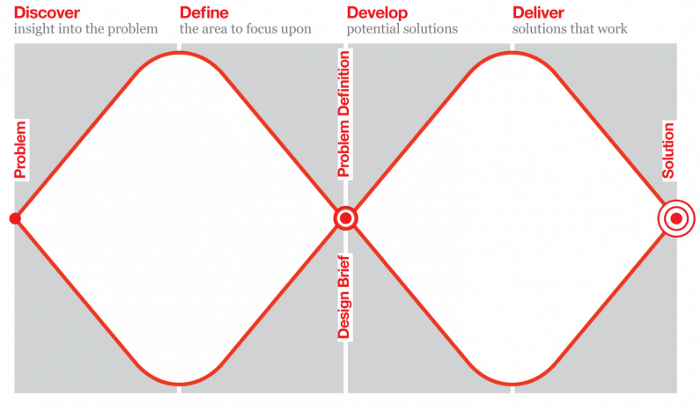
\includegraphics[width=1.0\textwidth]{img/double-diamond}
  \centering
  \caption{Design Thinking mithilfe von Double Diamond}
\end{figure}
  
\subsection{Risikomanagement}
\label{sec:risikomanagement}
Das Risikomanagement wurde iterativ-inkrementell jede Woche in den Stand-Ups durchgeführt. Dazu wurde ein Excel-Template verwendet, welche als Datei dem Anhang beigelegt wird. In diesem Template wurde jedem Risiko einen Risk Score zugeteilt, welcher sich aus Eintrittshäufigkeit multipliziert mit Schadensausmass errechnet. Anhand dieses Risk Scores wurde eine Risikomatrix erstellt, welche in Abbildung \ref{fig:risk-matrix} ersichtlich ist. Dieser Risk Score wurde vor und nach der definierten Prävention berechnet (siehe Abbildung \ref{fig:risk-matrix-after-measures}). Nachfolgend in der Tabelle \ref{tab:risikomanagement} werden lediglich die wichtigsten technischen Risiken und deren präventiven Massnahmen aufgelistet. 

\begin{center}
\begin{table}[H]
    \begin{tabularx}{\textwidth}{|l|X|X|}
        \hline
        \textbf{ID} & \textbf{Titel} & \textbf{Vorbeugende Massnahmen} \\ \hline
        R6 & Hindernisse werden nicht erkannt & Möglichst früh Konzept erstellen und mithilfe eines Prototyps testen. \\ \hline
        R8 & Roboter erfüllt 4 min Laufzeit nicht & Zeitbudget für einzelne Zustände im Gesamtablauf erstellen und in Evaluation mit einbeziehen. \\ \hline
        R9 & Komponenten lassen sich nicht kombinieren & Kompatibilität der verschiedenen Komponenten in die Evaluation mit einbeziehen \\ \hline
        R10 & Roboter kommt bei seitlicher Traversierung auf der Treppenstufe vom Kurs ab.& Orientierung auf einer Stufe in der Konzeption miteinbeziehen, früh Tests mit Prototypen durchführen.\\ \hline
        R11 & Fortbewegungskonzept wird durch die Beschaffenheit der Treppe gestört & Bei Evaluation Untergrund miteinbeziehen. Funktionsmuster bauen bei Unsicherheit. \\ \hline
        R12 & Der Roboter gerät bei der Hubbewegung aus dem Gleichgewicht. & Berechnung des Gewichts und des Schwerpunktes.\\ \hline
        R15 & Anschlag bei Drehbewegung in der Nähe eines Hindernisses bei minimalem Durchgang von 400 mm. & Lösungskonzept erarbeiten oder Dimension so wählen, dass Rotation immer möglich ist. \\ \hline
        R16 & Standfusspostition nach dem Einfahren der Ausleger nicht mehr richtig. & Ansteuerung der Motoren so justieren, dass Ausleger immer richtig eingefahren werden. \\ \hline
        R17 & Nicht alle Aspekte bei der Berechnung der Hubbewegung miteinkalkuliert. Hubbewegung funktioniert nicht. & Genaue Berechnungen, Prinzip belegen anhand Funktionsmuster.\\ \hline
        R18 & Hindernisse werden nicht erkannt. & Früh im PREN2 testen und Lichtverhältnisse miteinkalkulieren.\\ \hline
    \end{tabularx}
    \caption{Risikomanagement}
    \label{tab:risikomanagement}
\end{table}
\end{center}

\begin{figure}[H]
  \centering
  \begin{minipage}[t]{0.45\linewidth}
  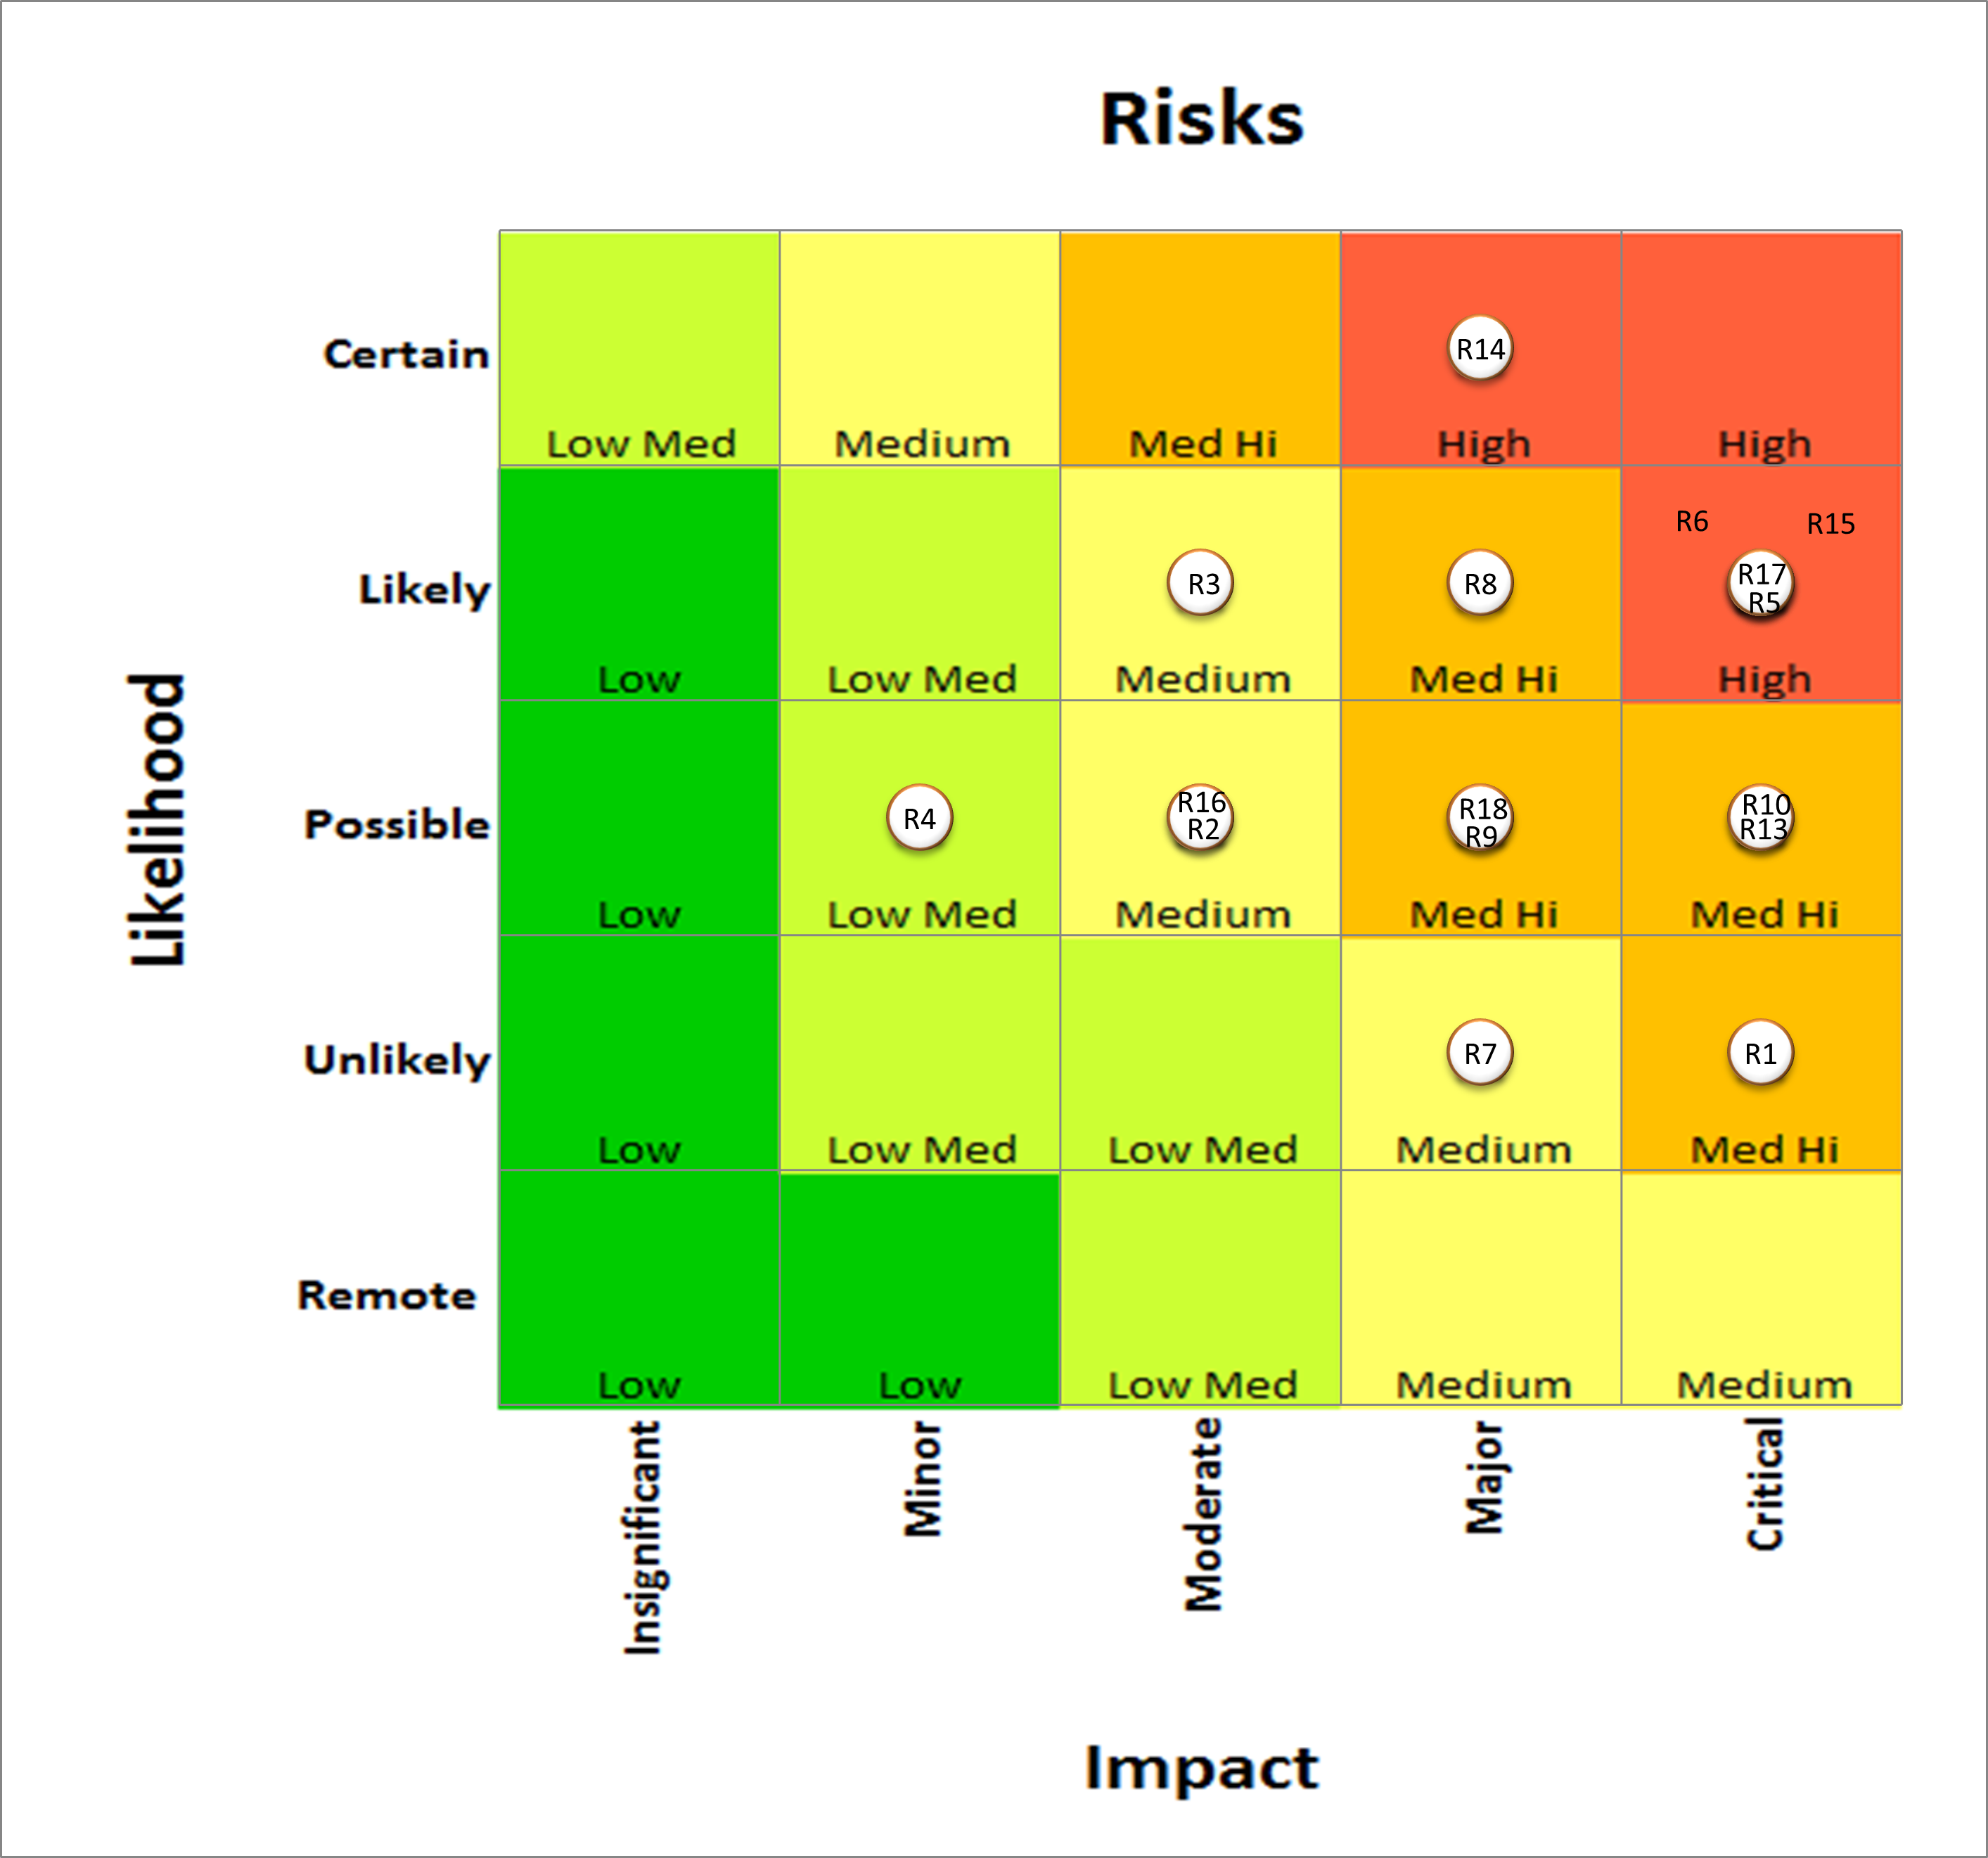
\includegraphics[width=1.0\textwidth]{img/risikomanagement/Risks.png}
  \caption{Risikomatrix}
  \label{fig:risk-matrix}
  \end{minipage} 
  \hfill
  \begin{minipage}[t]{0.45\linewidth}
  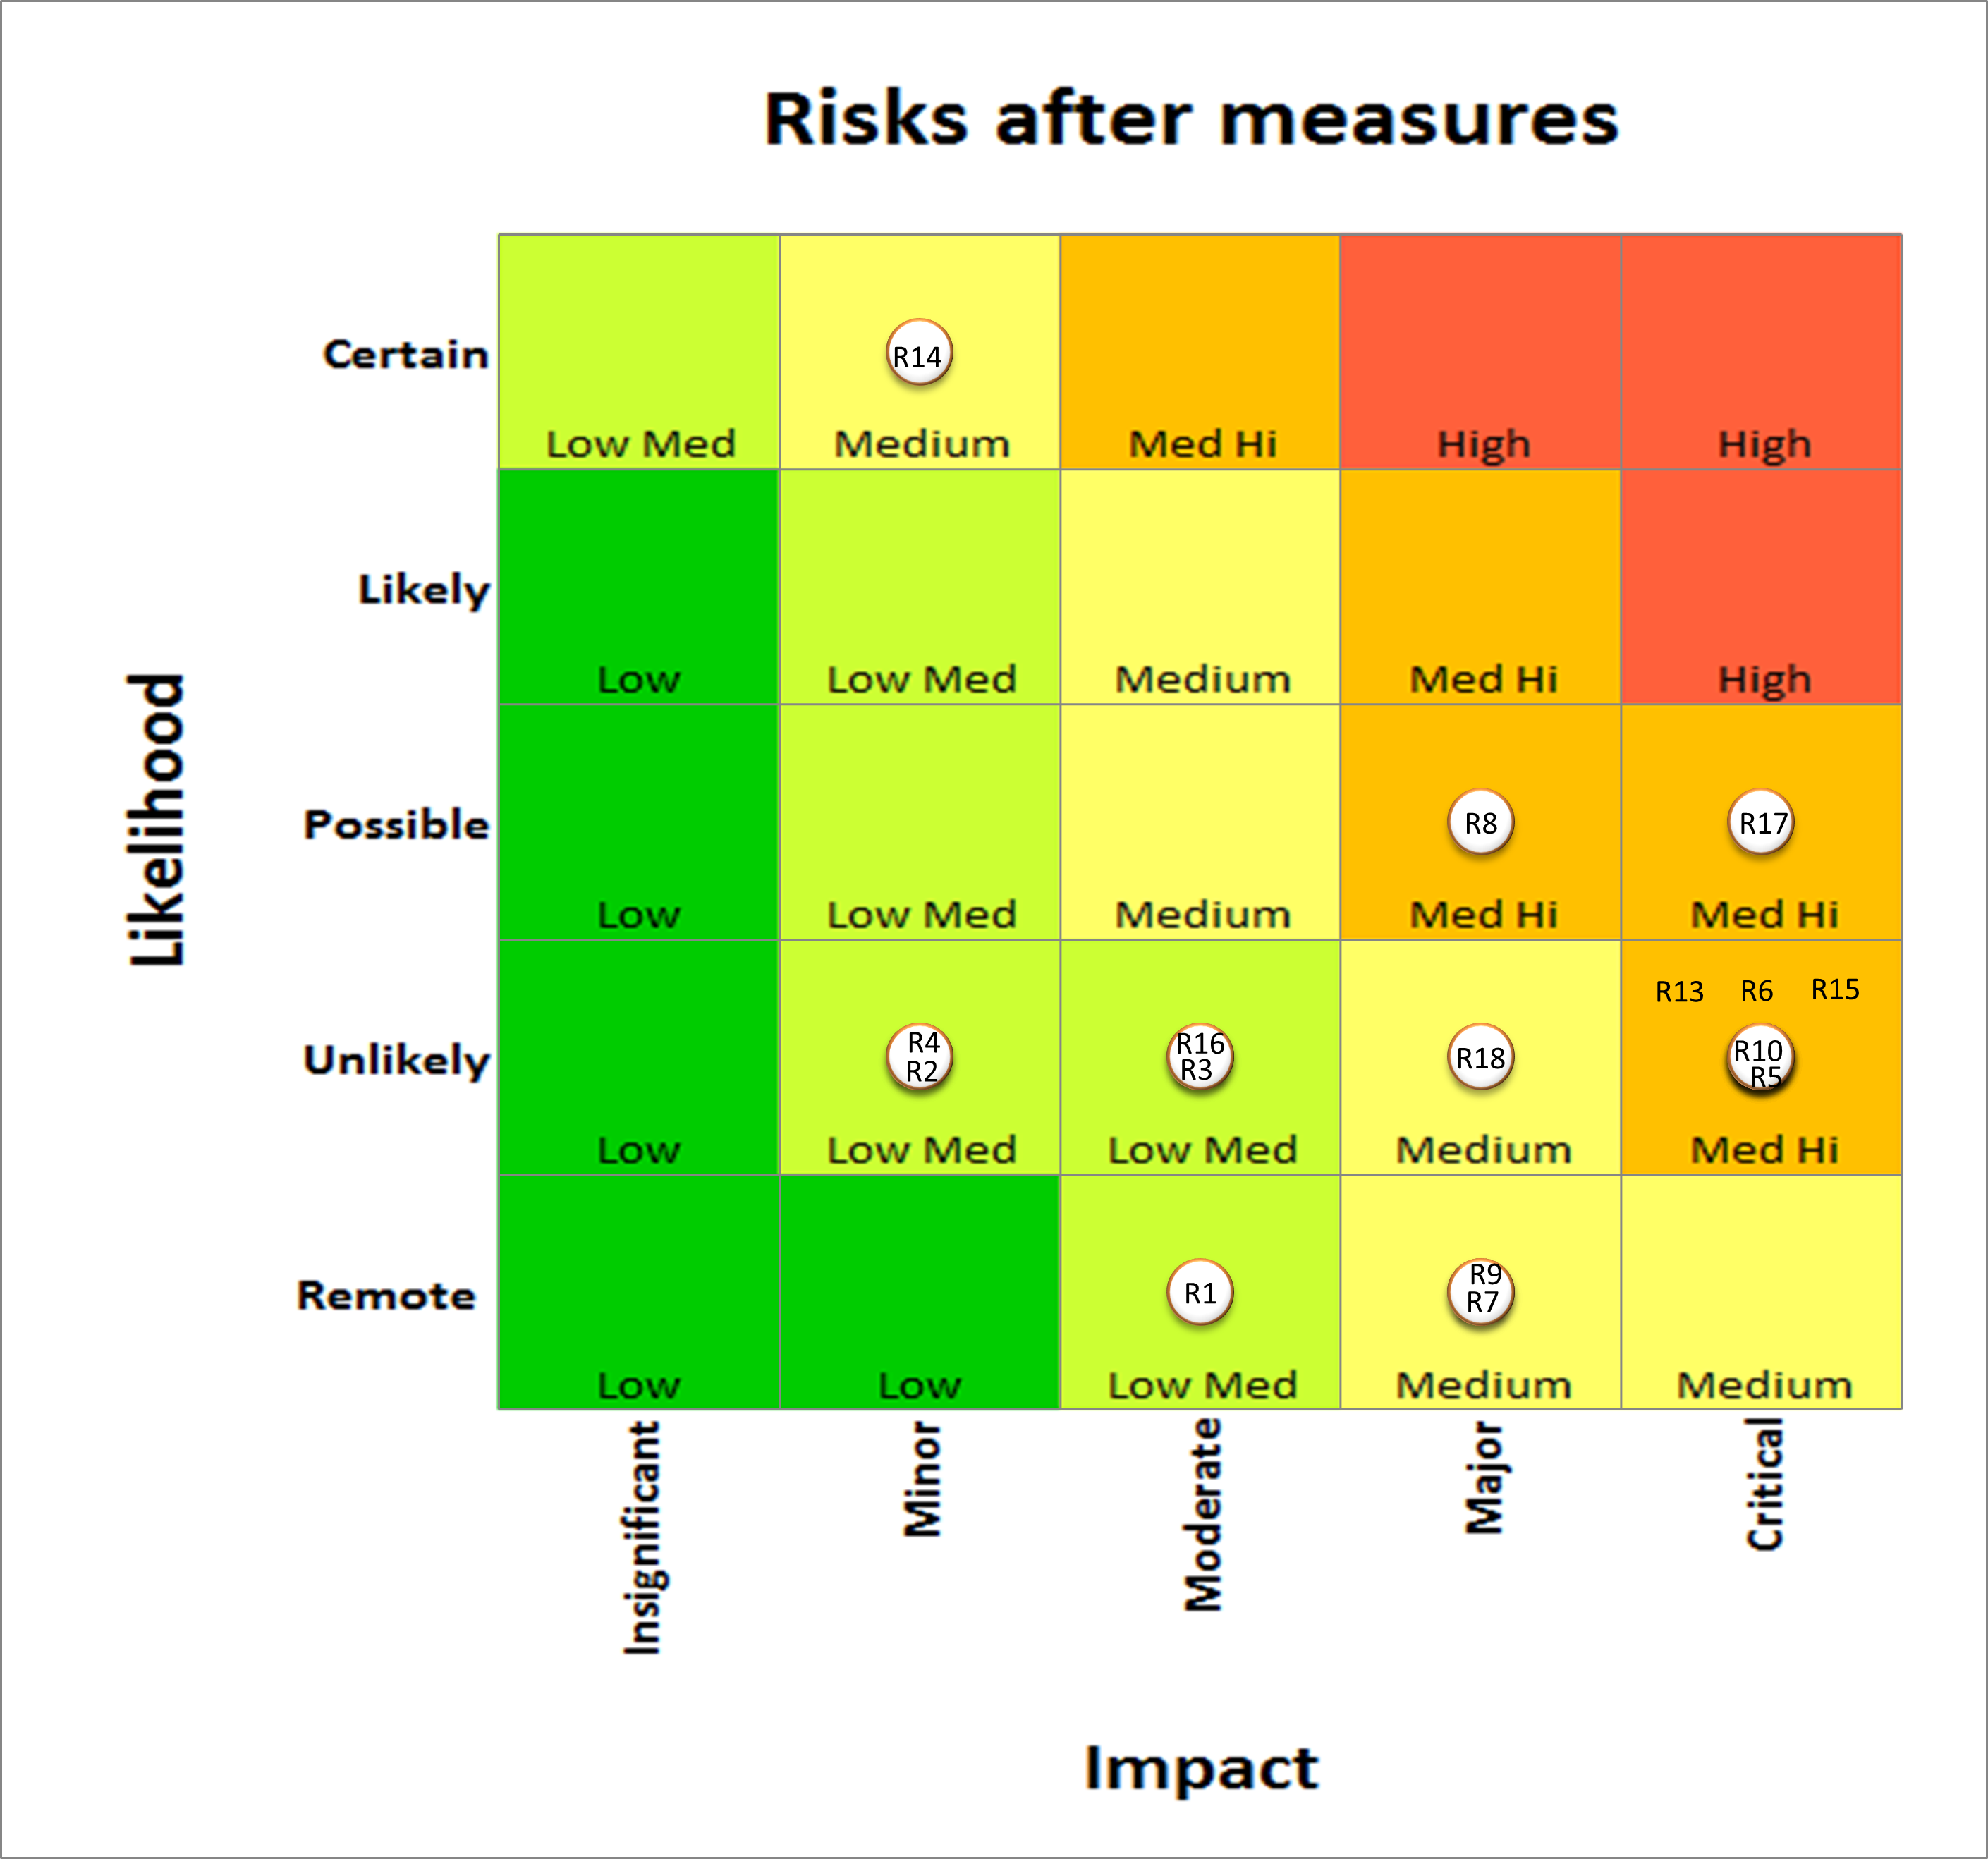
\includegraphics[width=1.0\textwidth]{img/risikomanagement/RisksAfterMeasures.png}
  \caption{Risikomatrix nach den präventiven Massnahmen}
  \label{fig:risk-matrix-after-measures}
  \end{minipage}
\end{figure}
  
\subsection{Rahmenplan}
Wie in Abbildung \ref{fig:rahmenplan} ersichtlich, hat sich das Team entschieden, das Projekt in vier Sprints aufzuteilen. Somit bilden die drei Testate und die Schlussabgabe die Ergebnisse, welche am Ende eines Sprints vorliegen sollen.

\begin{figure}[H]
  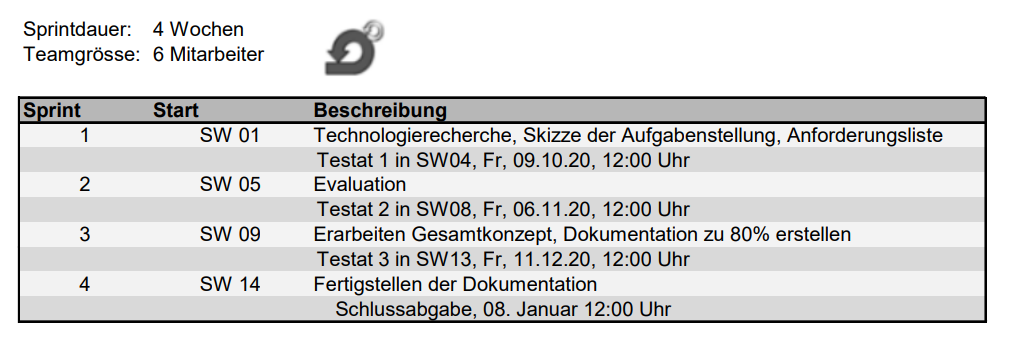
\includegraphics[width=1.0\textwidth]{img/projektmanagement/Rahmenplan.PNG}
  \centering
  \caption{Rahmenplan des Projekts}
  \label{fig:rahmenplan}
\end{figure}

\newpage

\subsection{Productbacklog}
Als zentrales Projektmanagement Element wurde ein Productbacklog aufgesetzt. Dieser dient als Übersicht, darüber, was in den nächsten Sprints getan werden muss. Da das \acrshort{pren1} Projekt jedoch in einem klar vorgegebenen Zeitrahmen steckt, das Endresultat klar definiert und auch das Budget fixiert ist, wurden bereits zu Beginn alle vier Sprints aufgelistet und grob geplant. 

\begin{figure}[H]
  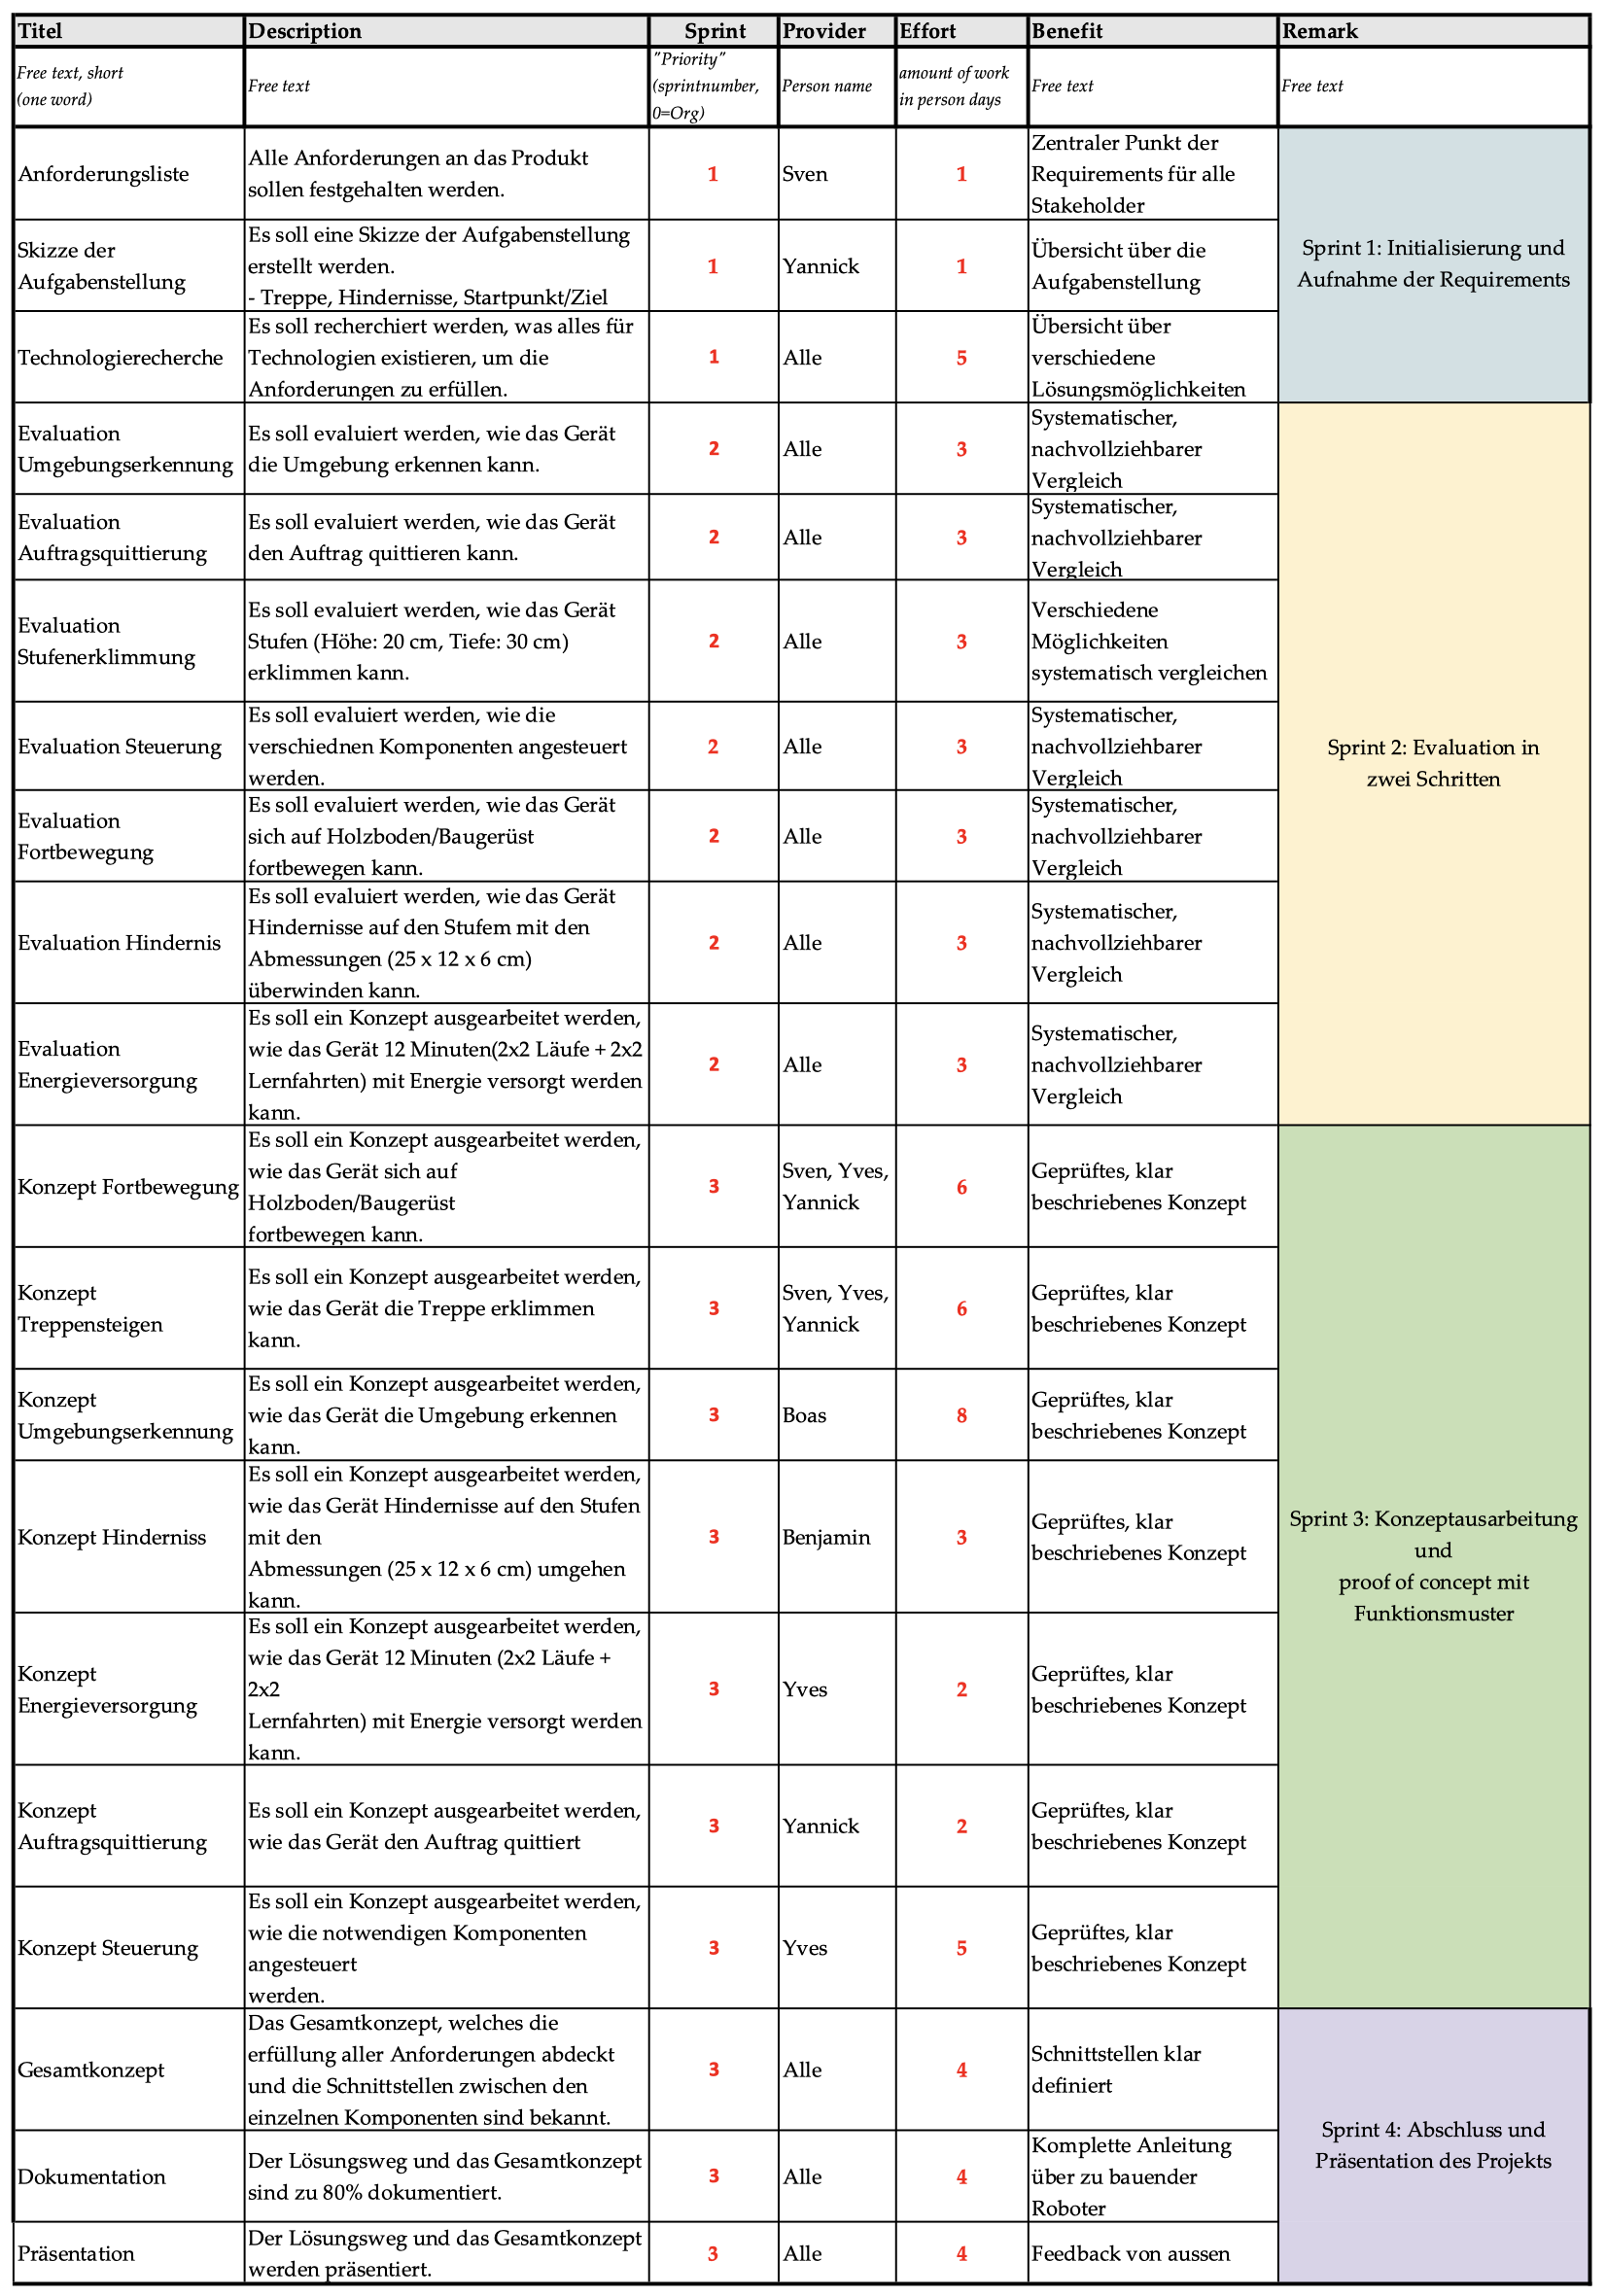
\includegraphics[width=0.95\textwidth]{img/projektmanagement/Backlog.png}
  \centering
  \caption{Productbacklog}
  \label{fig:productbacklog}
\end{figure}


\subsection{Sprintplanung}
Zu Beginn jedes Sprints wurde eine Sprintplanung gemacht. Dazu wurden die Backlog-Items (Epics) mit der höchsten Priorisierung in User-Storys aufgesplittet und in den Sprintbacklog übernommen. 

\subsubsection{Sprint 1}
\textbf{Sprintziel}\\
Das Ziel des Sprint 1 ist, den Roboter in Teilfunktionen zu unterteilen. Weiter soll eine Anforderungsliste und eine Skizze der Aufgabenstellung erstellt werden. Zudem sollen Recherchen bezüglich den einzelnen Teilfunktionen gemacht werden.

\textbf{Risiko-Update}\\
Es sind vier neue Risiken hinzugekommen. Nämlich, dass zu spät mit der Konzeption gestartet wird (R1), dass das Budget überschritten wird (R2), dass nicht fortlaufend dokumentiert wird (R3) und dass sich die Treppendimension ändert (R4).

\textbf{Sprintbacklog}\\
In der Abbildung \ref{fig:sprint-backlog-1} wird der Sprintbacklog gezeigt, welcher in der Sprintplanung erstellt wurde.
\begin{figure}[H]
  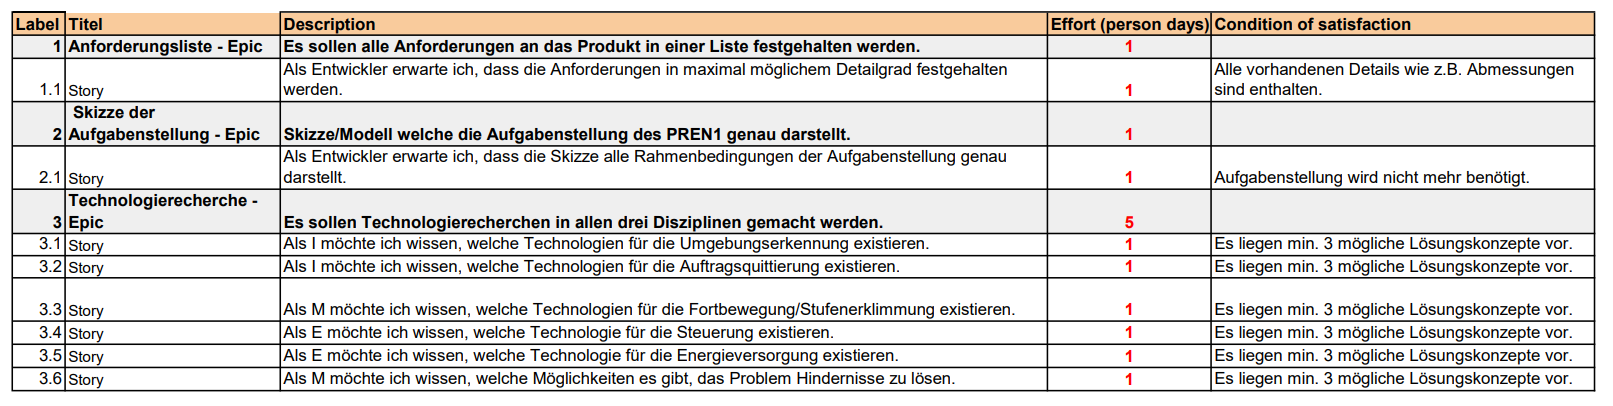
\includegraphics[angle=270,width=0.3\textwidth]{img/projektmanagement/sprint1-backlog.PNG}
  \centering
  \caption{Sprint 1 - Backlog}
  \label{fig:sprint-backlog-1}
\end{figure}

\newpage

\textbf{Sprintreview}\\
Das Sprintreview befindet sich im Anhang unter dem Abschnitt Arbeitsjournal - Technologierecherche und Anforderungsliste.


\subsubsection{Sprint 2}
\textbf{Sprintziel}\\
Das Ziel des Sprint 2 ist es, die verschiedenen Lösungsmöglichkeiten welche in Sprint 1 erarbeitet wurden einzugrenzen. Am Ende sollen drei mögliche Grobkonzepte stehen und ein klarer Favorit vorliegen.

\textbf{Risiko-Update}\\
Das Risiko R4, dass sich die Treppendimension ändert ist weggefallen. Da die Treppendimensionen klar spezifiziert und so versichert wurden. Die Risiken, einer Fehlerhaften Evaluation (R5), dass die Hindernisse nicht erkannt werden (R6), dass sich das Team zu früh auf eine Lösung fixiert (R7) und dass der Roboter die maximale Laufzeit von 4 min überschreitet (R8) sind hinzugekommen.

\textbf{Sprintbacklog}\\
In der Abbildung \ref{fig:sprint-backlog-2} wird der Sprintbacklog gezeigt, welcher in der Sprintplanung erstellt wurde.
\begin{figure}[H]
  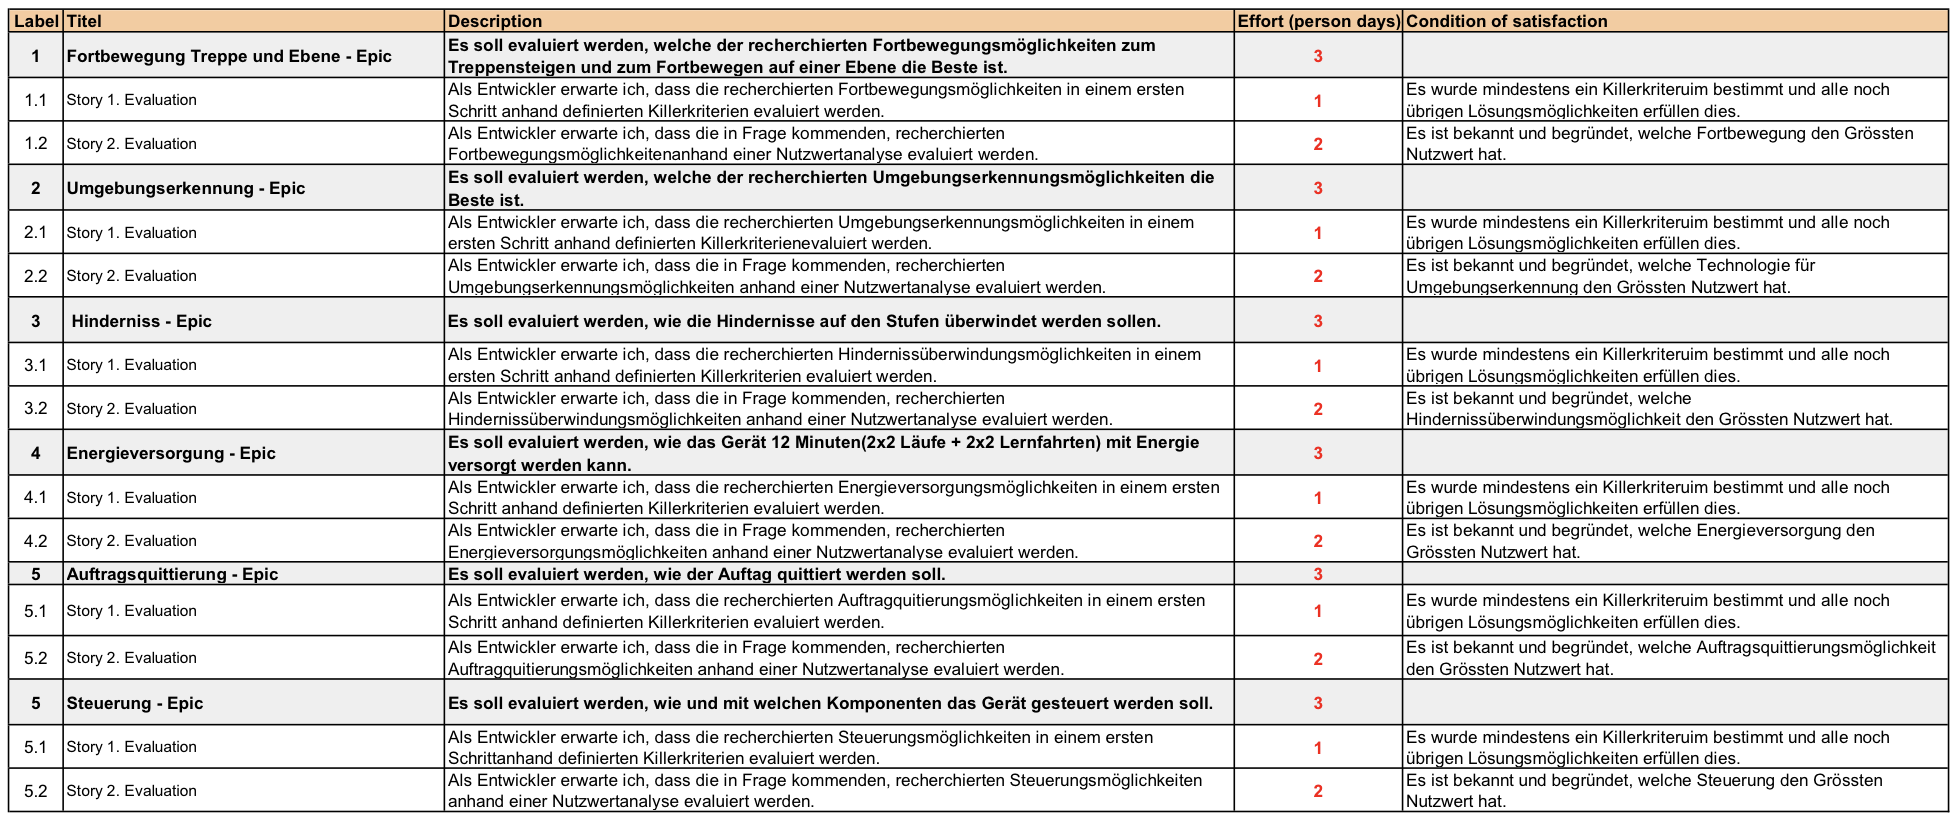
\includegraphics[angle=270,width=0.55\textwidth]{img/projektmanagement/sprint2-backlog2.png}
  \centering
  \caption{Sprint 2 - Backlog}
  \label{fig:sprint-backlog-2}
\end{figure}

\textbf{Sprintreview}\\
Das Sprintreview befindet sich im Anhang unter dem Abschnitt Arbeitsjournal - Evaluation, Auswahl der optimalen Lösungskombination(en).

\subsubsection{Sprint 3}
\textbf{Sprintziel}\\
Das Ziel des Sprint 3 ist, dass am Ende ein Gesamtkonzept vorliegt. Die Funktionsfähigkeit dieses Konzept ist mit Funktionsmuster untermauert.

\textbf{Risiko-Update}\\
Es sind keine Risiken weggefallen, jedoch neue hinzugekommen. Nämlich, dass sich die Komponenten nicht kombinieren lassen (R9), dass der Roboter beim seitlichen Verschieben eine Treppenstufe runter stürzt (R10), dass das Fortbewegungskonzept nicht mit der Oberflächenbeschaffenheit der Treppe zurecht kommt (R11), dass der Roboter bei der Hubbewegung aus dem Gleichgewicht fällt (R12), dass Teammitglieder aufgrund von Corona ausfallen (R13).

\textbf{Sprintbacklog}\\
In der Abbildung \ref{fig:sprint-backlog-3} wird der Sprintbacklog gezeigt, welcher in der Sprintplanung erstellt wurde.
\begin{figure}[H]
  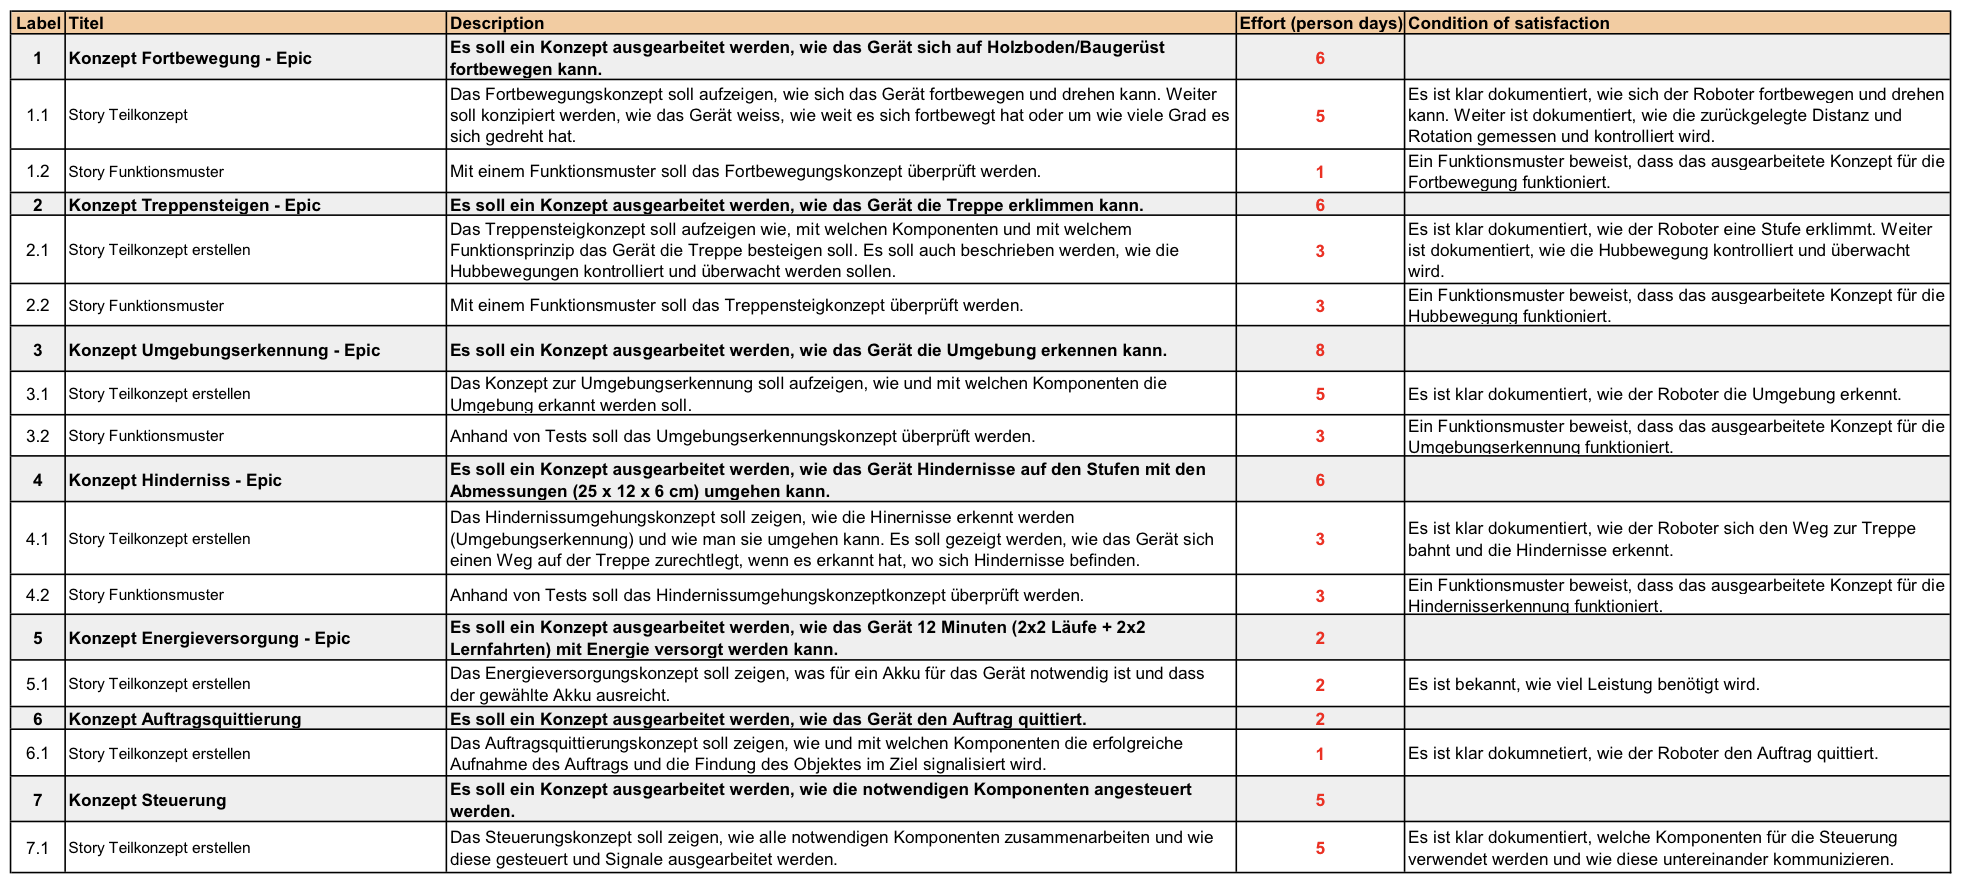
\includegraphics[angle=270,width=0.6\textwidth]{img/projektmanagement/sprint3-backlog2.png}
  \centering
  \caption{Sprint 3 - Backlog}
  \label{fig:sprint-backlog-3}
\end{figure}

\textbf{Sprintreview}\\
Das Sprintreview befindet sich im Anhang unter dem Abschnitt Arbeitsjournal - Freigabe des Gesamtkonzeptes, Dokumentation zu 80\% erstellt.

\subsubsection{Sprint 4}
\textbf{Sprintziel}\\
Das Ziel des Sprint 4 ist die fertige Dokumentation gemäss Kriterien.

\textbf{Risiko-Update}\\
Die Risiken R1 und R3 sind weggefallen, da die Dokumentation zu 80\% fertiggestellt und die Evaluation abgeschlossen ist. Neu hinzugekommen ist, dass sich der Roboter beim Drehen auf der Treppe in einem Hinderniss einhakt, wenn der Durchgang die minimal mögliche Breite von 400 mm hat (R14).

\textbf{Sprintbacklog}\\
Für den Sprint 4 wurde kein Sprintbacklog erstellt. Da es im Backlog keine weiteren Items mehr gab.

